\chapter{Proposed Model}\label{ch:proposed_model}
\epigraph{\textit{\normalsize “Artificial intelligence, in fact, is obviously an intelligence transmitted by conscious subjects, an intelligence placed in equipment.”}}{\textit{ \normalsize Pope Benedict XVI}}

\section{Generator} % (fold)
\label{sec:generator}
We use a deep convolutional generator model, this is similar to what DCGAN uses as generator. It starts with latent vector or noise of shape (100) which connects to a densely connected layer. We then use Reshape layer which reshapes it to (8, 8, 128) and perform batch normalization in batch normalization layer. We then perform up-sampling by using DeConv layer. DeConv layer is internally created by a up-sampling layer and Convolutional layer. We perform DeConv two more times to get the shape of the image as expected.
\begin{figure}[H]
\centering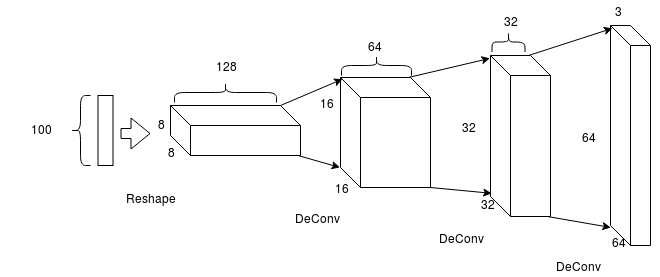
\includegraphics[width=1\textwidth]{images/Generator.png}
\caption{Generator architecture}
\label{fig:generator}
\end{figure} 

% section generator (end)








% _________________________________________________________________
% Layer (type)                 Output Shape              Param #   
% =================================================================
% dense_5 (Dense)              (None, 8192)              827392    
% _________________________________________________________________
% reshape_1 (Reshape)          (None, 8, 8, 128)         0         
% _________________________________________________________________
% batch_normalization_3 (Batch (None, 8, 8, 128)         512       
% _________________________________________________________________
% up_sampling2d_1 (UpSampling2 (None, 16, 16, 128)       0         
% _________________________________________________________________
% conv2d_1 (Conv2D)            (None, 16, 16, 128)       147584    
% _________________________________________________________________
% activation_1 (Activation)    (None, 16, 16, 128)       0         
% _________________________________________________________________
% batch_normalization_4 (Batch (None, 16, 16, 128)       512       
% _________________________________________________________________
% up_sampling2d_2 (UpSampling2 (None, 32, 32, 128)       0         
% _________________________________________________________________
% conv2d_2 (Conv2D)            (None, 32, 32, 64)        73792     
% _________________________________________________________________
% activation_2 (Activation)    (None, 32, 32, 64)        0         
% _________________________________________________________________
% batch_normalization_5 (Batch (None, 32, 32, 64)        256       
% _________________________________________________________________
% up_sampling2d_3 (UpSampling2 (None, 64, 64, 64)        0         
% _________________________________________________________________
% conv2d_3 (Conv2D)            (None, 64, 64, 32)        18464     
% _________________________________________________________________
% activation_3 (Activation)    (None, 64, 64, 32)        0         
% _________________________________________________________________
% batch_normalization_6 (Batch (None, 64, 64, 32)        128       
% _________________________________________________________________
% conv2d_4 (Conv2D)            (None, 64, 64, 3)         867       
% _________________________________________________________________
% activation_4 (Activation)    (None, 64, 64, 3)         0         
% =================================================================
% Total params: 1,069,507
% Trainable params: 1,068,803
% Non-trainable params: 704
% \begin{lstlisting}[basicstyle=\scriptsize,]
% __________________________________________________________________________________________________
% Layer (type)                    Output Shape         Param #     Connected to                     
% ==================================================================================================
% input_1 (InputLayer)            (None, 64, 64, 3)    0                                            
% __________________________________________________________________________________________________
% conv1 (Conv2D)                  (None, 56, 56, 256)  62464       input_1[0][0]                    
% __________________________________________________________________________________________________
% leaky_re_lu_1 (LeakyReLU)       (None, 56, 56, 256)  0           conv1[0][0]                      
% __________________________________________________________________________________________________
% batch_normalization_1 (BatchNor (None, 56, 56, 256)  1024        leaky_re_lu_1[0][0]              
% __________________________________________________________________________________________________
% primarycap_conv2 (Conv2D)       (None, 24, 24, 256)  5308672     batch_normalization_1[0][0]      
% __________________________________________________________________________________________________
% primarycap_reshape (Reshape)    (None, 18432, 8)     0           primarycap_conv2[0][0]           
% __________________________________________________________________________________________________
% primarycap_squash (Lambda)      (None, 18432, 8)     0           primarycap_reshape[0][0]         
% __________________________________________________________________________________________________
% batch_normalization_2 (BatchNor (None, 18432, 8)     32          primarycap_squash[0][0]          
% __________________________________________________________________________________________________
% flatten_1 (Flatten)             (None, 147456)       0           batch_normalization_2[0][0]      
% __________________________________________________________________________________________________
% uhat_digitcaps (Dense)          (None, 160)          23593120    flatten_1[0][0]                  
% __________________________________________________________________________________________________
% softmax_digitcaps1 (Activation) (None, 160)          0           uhat_digitcaps[0][0]             
% __________________________________________________________________________________________________
% dense_1 (Dense)                 (None, 160)          25760       softmax_digitcaps1[0][0]         
% __________________________________________________________________________________________________
% multiply_1 (Multiply)           (None, 160)          0           uhat_digitcaps[0][0]             
%                                                                  dense_1[0][0]                    
% __________________________________________________________________________________________________
% leaky_re_lu_2 (LeakyReLU)       (None, 160)          0           multiply_1[0][0]                 
% __________________________________________________________________________________________________
% softmax_digitcaps2 (Activation) (None, 160)          0           leaky_re_lu_2[0][0]              
% __________________________________________________________________________________________________
% dense_2 (Dense)                 (None, 160)          25760       softmax_digitcaps2[0][0]         
% __________________________________________________________________________________________________
% multiply_2 (Multiply)           (None, 160)          0           uhat_digitcaps[0][0]             
%                                                                  dense_2[0][0]                    
% __________________________________________________________________________________________________
% leaky_re_lu_3 (LeakyReLU)       (None, 160)          0           multiply_2[0][0]                 
% __________________________________________________________________________________________________
% softmax_digitcaps3 (Activation) (None, 160)          0           leaky_re_lu_3[0][0]              
% __________________________________________________________________________________________________
% dense_3 (Dense)                 (None, 160)          25760       softmax_digitcaps3[0][0]         
% __________________________________________________________________________________________________
% multiply_3 (Multiply)           (None, 160)          0           uhat_digitcaps[0][0]             
%                                                                  dense_3[0][0]                    
% __________________________________________________________________________________________________
% leaky_re_lu_4 (LeakyReLU)       (None, 160)          0           multiply_3[0][0]                 
% __________________________________________________________________________________________________
% dense_4 (Dense)                 (None, 1)            161         leaky_re_lu_4[0][0]              
% ==================================================================================================
% Total params: 29,042,753
% Trainable params: 29,042,225
% Non-trainable params: 528
% __________________________________________________________________________________________________
% \end{lstlisting}
